\chapter{极限与连续}

\section{极限的定义}

\begin{definition}[函数的极限]
设函数 \( f(x) \) 在点 \( x_0 \) 的某个去心邻域内有定义,如果存在常数 \( A \),对于任意给定的正数 \( \varepsilon \)(无论多么小),总存在正数 \( \delta \) 使得当 \( 0 < |x - x_0| < \delta \) 时,有 \( |f(x) - A| < \varepsilon \),那么常数 \( A \) 就叫做函数 \( f(x) \) 当 \( x \to x_0 \) 时的极限,记作
\[ \lim_{x \to x_0} f(x) = A \]
\end{definition}

\begin{example}
证明 \( \lim_{x \to 1} (2x + 1) = 3 \).
\end{example}

\begin{proof}
对于任意 \( \varepsilon > 0 \),取 \( \delta = \frac{\varepsilon}{2} \),则当 \( 0 < |x - 1| < \delta \) 时,
\[ |(2x + 1) - 3| = |2x - 2| = 2|x - 1| < 2\delta = \varepsilon \]
因此,由定义可知 \( \lim_{x \to 1} (2x + 1) = 3 \).
\end{proof}

\section{连续函数}

\begin{definition}[连续]
设函数 \( f(x) \) 在点 \( x_0 \) 的某个邻域内有定义,如果
\[ \lim_{x \to x_0} f(x) = f(x_0) \]
则称函数 \( f(x) \) 在点 \( x_0 \) 处连续。
\end{definition}

\begin{theorem}[连续函数的性质]
如果函数 \( f(x) \) 和 \( g(x) \) 都在点 \( x_0 \) 处连续,则它们的和、差、积、商(分母不为零)都在点 \( x_0 \) 处连续。
\end{theorem}

% 图片插入示例(注释掉,避免报错)
% \begin{figure}[htbp]
%     \centering
%     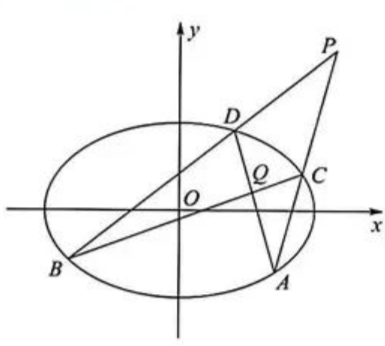
\includegraphics[width=0.6\textwidth]{flg/example.png}
%     \caption{函数的连续性示意图}
%     \label{fig:continuity}
% \end{figure}